\clearpage\begingroup\SourceLeaf{84b}\HistoricalHead{79}{R}{GAUSS AN OLBERS.}
\newcommand{\HistoricalCurrencyLSeven}{%
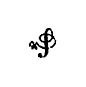
\begin{tikzpicture}[x=.1pt,y=-.1pt,baseline=-8pt]
\path[use as bounding box] (0,0) rectangle (110,112);
\path[fill=black,even odd rule]
(82,2) -- (72,2) -- (69,3) -- (65,7) -- (65,11) -- (61,17) -- (61,20) -- (60,21) -- (57,21) -- (55,23) -- (49,23) -- (49,25) -- (47,27) -- (45,27) -- (45,29) -- (40,34) -- (41,36) -- (40,41) -- (43,43) -- (43,45) -- (51,53) -- (56,53) -- (61,58) -- (59,60) -- (61,61) -- (61,71) -- (60,72) -- (54,68) -- (51,68) -- (48,65) -- (44,65) -- (41,62) -- (41,60) -- (35,54) -- (35,52) -- (33,50) -- (31,50) -- (31,52) -- (29,54) -- (29,56) -- (27,58) -- (26,61) -- (24,59) -- (23,53) -- (18,48) -- (14,48) -- (11,50) -- (11,52) -- (9,54) -- (7,54) -- (7,56) -- (5,58) -- (4,61) -- (5,63) -- (5,67) -- (7,69) -- (9,68) -- (12,68) -- (13,69) -- (13,77) -- (14,78) -- (21,78) -- (21,76) -- (23,74) -- (24,71) -- (25,72) -- (25,76) -- (27,78) -- (29,78) -- (31,80) -- (32,80) -- (33,78) -- (35,78) -- (35,72) -- (32,69) -- (32,67) -- (30,65) -- (30,61) -- (33,60) -- (34,62) -- (36,63) -- (36,65) -- (40,67) -- (40,69) -- (42,69) -- (43,71) -- (45,71) -- (47,73) -- (49,73) -- (55,77) -- (60,77) -- (63,80) -- (63,89) -- (61,90) -- (61,98) -- (57,104) -- (56,104) -- (50,98) -- (50,94) -- (48,92) -- (41,92) -- (41,93) -- (38,95) -- (38,105) -- (44,107) -- (45,109) -- (49,109) -- (51,107) -- (62,107) -- (65,104) -- (68,103) -- (68,101) -- (71,98) -- (73,92) -- (75,91) -- (75,78) -- (77,76) -- (75,74) -- (76,72) -- (73,69) -- (73,65) -- (75,64) -- (75,63) -- (73,62) -- (73,54) -- (74,53) -- (78,53) -- (80,51) -- (82,51) -- (86,47) -- (86,45) -- (92,39) -- (97,43) -- (97,55) -- (95,56) -- (95,58) -- (92,62) -- (90,63) -- (89,66) -- (87,66) -- (85,68) -- (82,68) -- (81,69) -- (81,71) -- (83,73) -- (89,73) -- (100,62) -- (100,60) -- (102,58) -- (102,49) -- (104,47) -- (98,42) -- (98,38) -- (96,36) -- (96,32) -- (94,30) -- (91,29) -- (91,15) -- (87,11) -- (86,6) -- cycle
(51,104) -- (53,102) -- (56,105) -- (53,106) -- cycle
(15,55) -- (17,57) -- (20,58) -- (20,62) -- (16,65) -- (13,65) -- (12,64) -- (12,58) -- cycle
(80,28) -- (82,30) -- (85,31) -- (86,33) -- (86,37) -- (80,45) -- (78,45) -- (74,48) -- (73,47) -- (73,43) -- (71,42) -- (71,40) -- (73,39) -- (72,37) -- (73,34) -- (71,33) -- (71,29) -- (72,28) -- cycle
(53,28) -- (60,28) -- (61,29) -- (61,31) -- (59,33) -- (59,38) -- (61,40) -- (59,42) -- (61,43) -- (61,47) -- (60,48) -- (54,48) -- (48,42) -- (48,36) -- (46,35) -- cycle
(78,6) -- (79,8) -- (85,13) -- (85,19) -- (86,20) -- (86,24) -- (85,25) -- (81,25) -- (80,23) -- (76,23) -- (74,21) -- (70,21) -- (69,20) -- (71,17) -- (71,15) -- (73,13) -- (73,11) -- (75,10) -- cycle
;
\end{tikzpicture}%
}

\begin{center}[7.]\end{center}
\begin{center}\textsc{Gauss} an \textsc{Olbers}.\quad Göttingen, 2. August 1832.\end{center}
\begin{center}
\rule{.74\textwidth}{.4pt}\\
{\small [\textsc{Wilhelm Olbers}, Sein Leben und seine Werke II, 2, 1910, S. 587 ff.]}\\[-.3ex]
\rule{.74\textwidth}{.4pt}
\end{center}
\noindent . . . . . . . . . . . . . . . . . . . . .\par
\indent Von jeher schien mir, dass die Apparate, deren man sich für die magnetischen
Bestimmungen bedient, sehr unvollkommen, und in einem schreienden
Misverhältnisse gegen die Schärfe unserer astronomischen und geodätischen
Messungen sind. Ich habe mir seit etwa 5 Monaten angelegen sein lassen,
diesem Übelstande abzuhelfen, wobei ich gleich anfangs von einigen schon
seit vielen Jahren gehabten Ideen ausging, aber freilich fast jede Woche noch
auf etwas Neues gekommen bin. Gegenwärtig habe ich zwei Apparate fertig
(ganz gleiche), womit absolute Declination und ihre Änderungen, Schwingungsdauer
etc. mit einer Schärfe gemessen werden können, die gar nichts zu wünschen
übrig lässt, angenommen für mich ein angemesseneres Local, wo kein
Eisen in der Nähe ist und jeder Luftzug abgehalten ist. Beides fehlt mir in
der Sternwarte und in meinem Hause, obwohl man den Einfluss davon auch
nicht überschätzen darf; auch so wie es jetzt ist, überbieten, meine ich, meine
Messungen alles Frühere \textls[120]{sehr} weit. Es ist hier aber eine sehr grosse Erndte
zu halten, und da ich, wenn der Himmel mir Leben und Kraft erhält, nicht
abgeneigt wäre, diesen Gegenständen ein eigenes Werk zu widmen, so wird
es damit, da ich stets alles Eilen mit Unreifem gehasst habe, wohl nicht so
ganz schnell gehen. Inzwischen habe ich die Absicht doch gleich eine Anwendung,
und zwar die allerwichtigste, in einer Societätsvorlesung bekannt zu
machen, nämlich die Bestimmung der absoluten Intensität des Erdmagnetis-
\clearpage\SourceLeaf{85}\HistoricalHead{80}{L}{PHYSIK. BRIEFWECHSEL.}
\noindent mus[\textsuperscript{*})].\begingroup\renewcommand{\thefootnote}{}
\footnotetext{[\textsuperscript{*}) \textit{Intensitas vis magneticae terrestris ad mensuram absolutam revocata},
1832, Werke V, S. 79.]}
\endgroup\ Ich habe schon, so wie meine Apparate sich nach und nach vervollkommneten,
eine beträchtliche Anzahl vorläufiger Versuche gemacht, und die
letzten werden der Wahrheit, soweit es in meinem Local möglich ist, schon
sehr nahe kommen; doch habe ich erst neulich wieder neue Vervollkommnungen
hinzugesetzt, nämlich Vorkehrungen, um alle Distanzmessungen dabei
mit \textls[120]{mikroskopischer} Schärfe auszuführen. Auch hierbei ist mir Freund
\textsc{Weber} durch Mittheilung seiner Hülfsmittel äusserst hilfreich gewesen.

Jene Vorlesung hoffe ich binnen einigen Monaten ausarbeiten zu können,
und einen kleinen Anfang habe ich bereits damit gemacht, indem ich eine
Einleitung aufgeschrieben habe, die das Wesentliche der Grundideen in einer
mehr populären Darstellung entwickelt. Es scheint, dass wenige Personen
hiervon bisher eine klare Vorstellung haben. Da es Sie vielleicht interessirt,
diese Einleitung zu lesen, so habe ich mein Brouillon abschreiben lassen
(\textsc{Harding} hat die Gefälligkeit gehabt), und ich lege solche Abschrift[\textsuperscript{**})]\begingroup\renewcommand{\thefootnote}{}
\footnotetext{[\textsuperscript{**}) Die Abschrift befindet sich nicht unter den Briefen.]}
\endgroup\ hier
bei. Bei der Bestimmung, welche der Aufsatz, wozu diese Einleitung gehört,
haben soll, ist es unnöthig zu bemerken, dass ich diese Mittheilung als \textls[120]{bloss}
\textls[120]{für Sie} bestimmt betrachten muss. Finden Sie, mein theurer \textsc{Olbers}, sich
aufgelegt, diesem Aufsatz Ihre Aufmerksamkeit zu schenken, und wünschen
über eines oder anderes darin weitere Aufklärung, so wird es mir die grösste
Freude sein, jeden Wink zu befolgen. Dieses Mal noch ein paar Worte über
die Schärfe meines Apparates.

Die absolute Declination wird mit grösster Leichtigkeit erhalten. Zwei
Secunden sind eine bestimmt sichtbar gemachte Grösse. Luftzug kann allerdings
bedeutend grössere Anomalien hineinbringen. Die tägliche Variation
kann man besonders in den Vormittagsstunden, wo sie am schnellsten ist,
schon nach einigen Zeitminuten sicher erkennen.

Bei Beobachtung der Schwingungsdauer einer Nadel lässt sich eine Schärfe
erreichen, die ich selbst früher für unglaublich gehalten haben würde. Die
Momente, wo eine Dauer zu Ende ist, haben nie einen Fehler von \(\frac{1}{10}\) Secunde,
sondern stets nur einige Hunderttheile. Ich beobachte nur kleine
Schwingungen, d. i. ich fange ungefähr da an, wo man sonst aufhörte, und
doch schwingt meine Nadel so, dass ich nach 6 oder 8 Stunden noch die
\clearpage\SourceLeaf{86}\HistoricalHead{81}{R}{GAUSS AN OLBERS.}\HistoricalFoot{XI1.}{11}
\noindent Momente mit grosser Sicherheit observire; habe ich eine neue Nadel eingehängt,
deren Schwingungsdauer noch unbekannt ist, so observire ich nur einige
wenige Schwingungen zu Anfang und kann dann getrost auf einige Stunden
in die Stadt gehen, wo nach meiner Zurückkunft von einer Ungewissheit,
wie \textls[120]{viele} Schwingungen unterdessen gemacht sind, gar keine Rede sein kann.
Ich habe sogar schon zuweilen bei Nacht etwas grössere Schwingungen eingeleitet,
aber nicht wie Herr \textsc{Quetelet} von \(60^{0}\), sondern z. B. von \(10^{0}\), wo
ich die Nadel bei Nacht ihrem Schicksal überlassen habe, und nach dem
Aufstehen am andern Morgen mit Sicherheit habe angeben können, wie viele
Schwingungen unterdessen gemacht sind.

Nichts desto weniger ist der modus prior (pag. 3) der Anlage dem
zweiten \textls[120]{bei weitem} nachzusetzen, und zwar deswegen, weil jener eine viel
längere Zeit erfordert, während welcher die \textls[120]{Veränderlichkeit} des Erdmagnetismus
sich auf das Entscheidenste bemerklich macht. Ich habe zwar
auch mehrere Versuche nach dem modus prior gemacht (die nahezu dieselben
Resultate geben), werde aber bei denen, die \textls[120]{gelten} sollen, mich nur
auf den zweiten Modus beschränken. Vielleicht interessirt es Sie, die Resultate
meiner letzten Versuche, obwohl solche immer erst als vorläufige zu betrachten
sind, kennen zu lernen.

Als Einheiten angenommen:
\begin{list}{}{\setlength{\leftmargin}{2.6em}\setlength{\labelwidth}{1.4em}\setlength{\labelsep}{.6em}\setlength{\itemsep}{0pt}\setlength{\parsep}{0pt}\setlength{\topsep}{.2ex}}
\item[1)] das Gewicht (i. e. die \textls[120]{Masse}), die man ein Milligramm nennt,
\item[2)] den Millimeter,
\item[3)] diejenige beschleunigende Kraft, die in der Zeitsekunde einen doppelten
Fall von 1 Millimeter hervorbringt (wobei also die Schwere in
Göttingen \(=9812\) ist),
\end{list}
\noindent ist die Intensität des horizontalen Theils des Erdmagnetismus in Göttingen
\begin{center}
nach Versuchen vom 22.—26. Juli mit\\[.4ex]
\begin{tabular}{@{}r@{\quad}c@{\quad}l@{}}
Nadel 1 & . . . . . & \(=1{,}7762\)\\
mit Nadel A & . . . . . & \(=1.7780\)\\[-.5ex]
&\multicolumn{2}{r@{}}{\rule{8em}{.4pt}}\\[-.5ex]
&im Mittel&\(1{,}7771\)\textsuperscript{*}),\\
\end{tabular}
\end{center}
\begingroup\renewcommand{\thefootnote}{}
\footnotetext{\textsuperscript{*}) Die Zahl bleibt dieselbe, wenn man respective das Gramm und den Meter als
Einheit ansieht.}\endgroup
\noindent wovon also die beiden einzelnen Resultate nicht viel mehr als den \(2000^{\text{ten}}\) Theil
\clearpage\SourceLeaf{87}\HistoricalHead{82}{L}{PHYSIK. BRIEFWECHSEL.}
\noindent abweichen. Die \textls[120]{Veränderung} der Intensität während eines Tages ist öfter
4mahl so gross.

Ein früherer Versuch, mit fast gleichen Attentionen gemacht, gab
\[
1{,}7650
\]
\noindent aber in einem anderen Local, wo eben die Localität sehr gut \(\frac{1}{2}\) p[ro]c[ent]
Unterschied leicht erklärt, da überall Eisen nicht zu vermeiden war. Ich werde
demnächst auch das Verhältniss der Intensität am ersteren Local zu der ganz
im Freien zu bestimmen versuchen.

Noch frühere Versuche, wobei aber manche Cautelen\textsuperscript{*})\begingroup\renewcommand{\thefootnote}{}
\footnotetext{\textsuperscript{*}) Z. B. auch wegen Torsion der Fäden.}\endgroup\ noch nicht genug
berücksichtigt waren, mit anderen Nadeln und in \textls[120]{andern Localen} gaben
\begin{center}
\begin{tabular}{@{}r@{\quad}c@{\quad}l@{}}
am 21. Mai & . . . . . & \(1{,}788\)\\
24. Mai & . . . . . & \(1{,}777\)\\
4. Juni & . . . . . & \(1{,}779\).
\end{tabular}
\end{center}
\noindent\hspace*{\parindent}Eine Menge von Untersuchungen habe ich mir noch vorgesetzt, die aber
einen grossen Aufwand von Zeit kosten werden, z. B. über den Einfluss der
Temperatur auf die Nadeln, über das allmähliche Abnehmen der magnetischen
Kraft in den Nadeln, wenn sie anfangs so stark wie möglich magnetisirt sind
und dann \textls[120]{theils mit, theils ohne} Armatur aufbewahrt werden, über das
Verhalten anderer Körper, ganz besonders des Argentans pp. Bei allen diesen
Geschäften wird mir die Hülfe des trefflichen \textsc{Weber} äusserst schätzbar sein. —
Vielleicht wird unser Gouvernement, wenn die Geldklemme nicht zu gross ist,
demnächst nicht abgeneigt sein, ein eigenes magnetisches Häuschen, worin gar
kein Eisen ist, zu errichten. Ich werde aber nicht eher darauf antragen, als
bis alle meine Vorarbeiten gehörig \textls[120]{reif} sind.

Noch durch einen Umstand empfehlen sich meine Einrichtungen. Meine
beiden ganz gleichen Apparate, die für \textls[120]{alle} Fragen, bloss die Inclination
ausgenommen, zureichen und die oben bezeichnete Schärfe geben, kosten
inclusive von 6 Stahlstäben, jeder fast 1 {\fontspec{FreeSerif.otf}℔} schwer, zusammen nur 81 \HistoricalCurrencyLSeven;
\textsc{Gambey}sche Apparate für absolute Declination, tägliche Variation, Schwingungsdauer,
während sie alles nur sehr unvollkommen leisten, würden vielleicht
zusammen, \textls[120]{jeder einfach}, fast 20mahl so viel kosten. Ich werde zunächst
\clearpage\SourceLeaf{88a}\HistoricalHead{83}{R}{GAUSS AN ENCKE}
\noindent noch eine Anzahl Stäbe aus Englischem Gussstahl verfertigen lassen, die, wie
meine Erfahrungen zeigen, nicht bloss stärkern Magnetismus annehmen, sondern
ihn auch zäher an sich halten, als Nadeln aus Cementstahl. . . . . . . . . . .
\clearpage\endgroup
